\documentclass[1p]{elsarticle_modified}
%\bibliographystyle{elsarticle-num}

%\usepackage[colorlinks]{hyperref}
%\usepackage{abbrmath_seonhwa} %\Abb, \Ascr, \Acal ,\Abf, \Afrak
\usepackage{amsfonts}
\usepackage{amssymb}
\usepackage{amsmath}
\usepackage{amsthm}
\usepackage{scalefnt}
\usepackage{amsbsy}
\usepackage{kotex}
\usepackage{caption}
\usepackage{subfig}
\usepackage{color}
\usepackage{graphicx}
\usepackage{xcolor} %% white, black, red, green, blue, cyan, magenta, yellow
\usepackage{float}
\usepackage{setspace}
\usepackage{hyperref}

\usepackage{tikz}
\usetikzlibrary{arrows}

\usepackage{multirow}
\usepackage{array} % fixed length table
\usepackage{hhline}

%%%%%%%%%%%%%%%%%%%%%
\makeatletter
\renewcommand*\env@matrix[1][\arraystretch]{%
	\edef\arraystretch{#1}%
	\hskip -\arraycolsep
	\let\@ifnextchar\new@ifnextchar
	\array{*\c@MaxMatrixCols c}}
\makeatother %https://tex.stackexchange.com/questions/14071/how-can-i-increase-the-line-spacing-in-a-matrix
%%%%%%%%%%%%%%%

\usepackage[normalem]{ulem}

\newcommand{\msout}[1]{\ifmmode\text{\sout{\ensuremath{#1}}}\else\sout{#1}\fi}
%SOURCE: \msout is \stkout macro in https://tex.stackexchange.com/questions/20609/strikeout-in-math-mode

\newcommand{\cancel}[1]{
	\ifmmode
	{\color{red}\msout{#1}}
	\else
	{\color{red}\sout{#1}}
	\fi
}

\newcommand{\add}[1]{
	{\color{blue}\uwave{#1}}
}

\newcommand{\replace}[2]{
	\ifmmode
	{\color{red}\msout{#1}}{\color{blue}\uwave{#2}}
	\else
	{\color{red}\sout{#1}}{\color{blue}\uwave{#2}}
	\fi
}

\newcommand{\Sol}{\mathcal{S}} %segment
\newcommand{\D}{D} %diagram
\newcommand{\A}{\mathcal{A}} %arc


%%%%%%%%%%%%%%%%%%%%%%%%%%%%%5 test

\def\sl{\operatorname{\textup{SL}}(2,\Cbb)}
\def\psl{\operatorname{\textup{PSL}}(2,\Cbb)}
\def\quan{\mkern 1mu \triangleright \mkern 1mu}

\theoremstyle{definition}
\newtheorem{thm}{Theorem}[section]
\newtheorem{prop}[thm]{Proposition}
\newtheorem{lem}[thm]{Lemma}
\newtheorem{ques}[thm]{Question}
\newtheorem{cor}[thm]{Corollary}
\newtheorem{defn}[thm]{Definition}
\newtheorem{exam}[thm]{Example}
\newtheorem{rmk}[thm]{Remark}
\newtheorem{alg}[thm]{Algorithm}

\newcommand{\I}{\sqrt{-1}}
\begin{document}

%\begin{frontmatter}
%
%\title{Boundary parabolic representations of knots up to 8 crossings}
%
%%% Group authors per affiliation:
%\author{Yunhi Cho} 
%\address{Department of Mathematics, University of Seoul, Seoul, Korea}
%\ead{yhcho@uos.ac.kr}
%
%
%\author{Seonhwa Kim} %\fnref{s_kim}}
%\address{Center for Geometry and Physics, Institute for Basic Science, Pohang, 37673, Korea}
%\ead{ryeona17@ibs.re.kr}
%
%\author{Hyuk Kim}
%\address{Department of Mathematical Sciences, Seoul National University, Seoul 08826, Korea}
%\ead{hyukkim@snu.ac.kr}
%
%\author{Seokbeom Yoon}
%\address{Department of Mathematical Sciences, Seoul National University, Seoul, 08826,  Korea}
%\ead{sbyoon15@snu.ac.kr}
%
%\begin{abstract}
%We find all boundary parabolic representation of knots up to 8 crossings.
%
%\end{abstract}
%\begin{keyword}
%    \MSC[2010] 57M25 
%\end{keyword}
%
%\end{frontmatter}

%\linenumbers
%\tableofcontents
%
\newcommand\colored[1]{\textcolor{white}{\rule[-0.35ex]{0.8em}{1.4ex}}\kern-0.8em\color{red} #1}%
%\newcommand\colored[1]{\textcolor{white}{ #1}\kern-2.17ex	\textcolor{white}{ #1}\kern-1.81ex	\textcolor{white}{ #1}\kern-2.15ex\color{red}#1	}

{\Large $\underline{11a_{254}~(K11a_{254})}$}

\setlength{\tabcolsep}{10pt}
\renewcommand{\arraystretch}{1.6}
\vspace{1cm}\begin{tabular}{m{100pt}>{\centering\arraybackslash}m{274pt}}
\multirow{5}{120pt}{
	\centering
	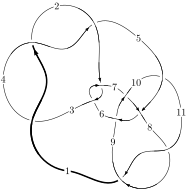
\includegraphics[width=112pt]{../../../GIT/diagram.site/Diagrams/png/503_11a_254.png}\\
\ \ \ A knot diagram\footnotemark}&
\allowdisplaybreaks
\textbf{Linearized knot diagam} \\
\cline{2-2}
 &
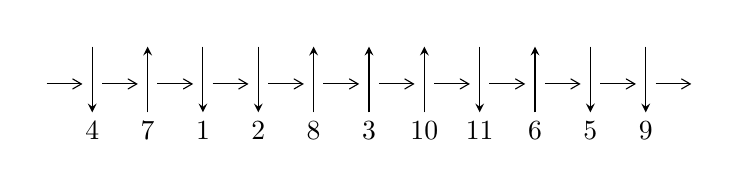
\begin{tikzpicture}[x=20pt, y=17pt]
	% nodes
	\node (C0) at (0, 0) {};
	\node (C1) at (1, 0) {};
	\node (C1U) at (1, +1) {};
	\node (C1D) at (1, -1) {4};

	\node (C2) at (2, 0) {};
	\node (C2U) at (2, +1) {};
	\node (C2D) at (2, -1) {7};

	\node (C3) at (3, 0) {};
	\node (C3U) at (3, +1) {};
	\node (C3D) at (3, -1) {1};

	\node (C4) at (4, 0) {};
	\node (C4U) at (4, +1) {};
	\node (C4D) at (4, -1) {2};

	\node (C5) at (5, 0) {};
	\node (C5U) at (5, +1) {};
	\node (C5D) at (5, -1) {8};

	\node (C6) at (6, 0) {};
	\node (C6U) at (6, +1) {};
	\node (C6D) at (6, -1) {3};

	\node (C7) at (7, 0) {};
	\node (C7U) at (7, +1) {};
	\node (C7D) at (7, -1) {10};

	\node (C8) at (8, 0) {};
	\node (C8U) at (8, +1) {};
	\node (C8D) at (8, -1) {11};

	\node (C9) at (9, 0) {};
	\node (C9U) at (9, +1) {};
	\node (C9D) at (9, -1) {6};

	\node (C10) at (10, 0) {};
	\node (C10U) at (10, +1) {};
	\node (C10D) at (10, -1) {5};

	\node (C11) at (11, 0) {};
	\node (C11U) at (11, +1) {};
	\node (C11D) at (11, -1) {9};
	\node (C12) at (12, 0) {};

	% arrows
	\draw[->,>={angle 60}]
	(C0) edge (C1) (C1) edge (C2) (C2) edge (C3) (C3) edge (C4) (C4) edge (C5) (C5) edge (C6) (C6) edge (C7) (C7) edge (C8) (C8) edge (C9) (C9) edge (C10) (C10) edge (C11) (C11) edge (C12) ;	\draw[->,>=stealth]
	(C1U) edge (C1D) (C2D) edge (C2U) (C3U) edge (C3D) (C4U) edge (C4D) (C5D) edge (C5U) (C6D) edge (C6U) (C7D) edge (C7U) (C8U) edge (C8D) (C9D) edge (C9U) (C10U) edge (C10D) (C11U) edge (C11D) ;
	\end{tikzpicture} \\
\hhline{~~} \\& 
\textbf{Solving Sequence} \\ \cline{2-2} 
 &
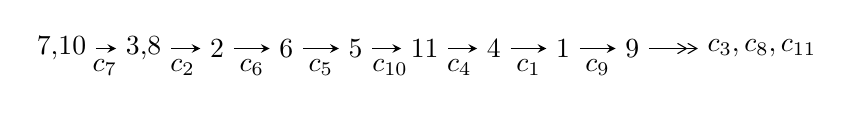
\begin{tikzpicture}[x=25pt, y=7pt]
	% node
	\node (A0) at (-1/8, 0) {7,10};
	\node (A1) at (17/16, 0) {3,8};
	\node (A2) at (17/8, 0) {2};
	\node (A3) at (25/8, 0) {6};
	\node (A4) at (33/8, 0) {5};
	\node (A5) at (41/8, 0) {11};
	\node (A6) at (49/8, 0) {4};
	\node (A7) at (57/8, 0) {1};
	\node (A8) at (65/8, 0) {9};
	\node (C1) at (1/2, -1) {$c_{7}$};
	\node (C2) at (13/8, -1) {$c_{2}$};
	\node (C3) at (21/8, -1) {$c_{6}$};
	\node (C4) at (29/8, -1) {$c_{5}$};
	\node (C5) at (37/8, -1) {$c_{10}$};
	\node (C6) at (45/8, -1) {$c_{4}$};
	\node (C7) at (53/8, -1) {$c_{1}$};
	\node (C8) at (61/8, -1) {$c_{9}$};
	\node (A9) at (10, 0) {$c_{3},c_{8},c_{11}$};

	% edge
	\draw[->,>=stealth]	
	(A0) edge (A1) (A1) edge (A2) (A2) edge (A3) (A3) edge (A4) (A4) edge (A5) (A5) edge (A6) (A6) edge (A7) (A7) edge (A8) ;
	\draw[->>,>={angle 60}]	
	(A8) edge (A9);
\end{tikzpicture} \\ 

\end{tabular} \\

\footnotetext{
The image of knot diagram is generated by the software ``\textbf{Draw programme}" developed by Andrew Bartholomew(\url{http://www.layer8.co.uk/maths/draw/index.htm\#Running-draw}), where we modified some parts for our purpose(\url{https://github.com/CATsTAILs/LinksPainter}).
}\phantom \\ \newline 
\centering \textbf{Ideals for irreducible components\footnotemark of $X_{\text{par}}$} 
 
\begin{align*}
I^u_{1}&=\langle 
-6.04159\times10^{241} u^{70}+7.02943\times10^{242} u^{69}+\cdots+6.12381\times10^{241} b+8.22545\times10^{241},\\
\phantom{I^u_{1}}&\phantom{= \langle  }2.08888\times10^{242} u^{70}-2.32560\times10^{243} u^{69}+\cdots+6.12381\times10^{241} a+2.43849\times10^{242},\;u^{71}-12 u^{70}+\cdots-2 u+1\rangle \\
I^u_{2}&=\langle 
b,\;- u^5+2 u^4+u^3-3 u^2+a+2,\;u^6- u^5- u^4+2 u^3- u+1\rangle \\
\\
\end{align*}
\raggedright * 2 irreducible components of $\dim_{\mathbb{C}}=0$, with total 77 representations.\\
\footnotetext{All coefficients of polynomials are rational numbers. But the coefficients are sometimes approximated in decimal forms when there is not enough margin.}
\newpage
\renewcommand{\arraystretch}{1}
\centering \section*{I. $I^u_{1}= \langle -6.04\times10^{241} u^{70}+7.03\times10^{242} u^{69}+\cdots+6.12\times10^{241} b+8.23\times10^{241},\;2.09\times10^{242} u^{70}-2.33\times10^{243} u^{69}+\cdots+6.12\times10^{241} a+2.44\times10^{242},\;u^{71}-12 u^{70}+\cdots-2 u+1 \rangle$}
\flushleft \textbf{(i) Arc colorings}\\
\begin{tabular}{m{7pt} m{180pt} m{7pt} m{180pt} }
\flushright $a_{7}=$&$\begin{pmatrix}1\\0\end{pmatrix}$ \\
\flushright $a_{10}=$&$\begin{pmatrix}0\\u\end{pmatrix}$ \\
\flushright $a_{3}=$&$\begin{pmatrix}-3.41108 u^{70}+37.9764 u^{69}+\cdots-4.41767 u-3.98199\\0.986573 u^{70}-11.4788 u^{69}+\cdots+1.16296 u-1.34319\end{pmatrix}$ \\
\flushright $a_{8}=$&$\begin{pmatrix}1\\- u^2\end{pmatrix}$ \\
\flushright $a_{2}=$&$\begin{pmatrix}-4.39765 u^{70}+49.4552 u^{69}+\cdots-5.58062 u-2.63880\\0.986573 u^{70}-11.4788 u^{69}+\cdots+1.16296 u-1.34319\end{pmatrix}$ \\
\flushright $a_{6}=$&$\begin{pmatrix}0.676294 u^{70}-8.31654 u^{69}+\cdots+9.11289 u-1.31962\\0.0427928 u^{70}-0.0844798 u^{69}+\cdots+0.876884 u+1.75188\end{pmatrix}$ \\
\flushright $a_{5}=$&$\begin{pmatrix}1.00267 u^{70}-12.5483 u^{69}+\cdots+9.31432 u-3.27251\\0.304306 u^{70}-3.13984 u^{69}+\cdots+1.83385 u+1.43659\end{pmatrix}$ \\
\flushright $a_{11}=$&$\begin{pmatrix}-1.46583 u^{70}+16.5432 u^{69}+\cdots-16.5616 u+9.43161\\0.491717 u^{70}-5.73898 u^{69}+\cdots+1.64593 u-1.66950\end{pmatrix}$ \\
\flushright $a_{4}=$&$\begin{pmatrix}3.16529 u^{70}-35.6825 u^{69}+\cdots+7.81990 u+2.97070\\-0.426948 u^{70}+5.06894 u^{69}+\cdots+0.0537692 u+1.02327\end{pmatrix}$ \\
\flushright $a_{1}=$&$\begin{pmatrix}-2.10032 u^{70}+24.1805 u^{69}+\cdots-0.598859 u+2.20095\\0.426948 u^{70}-5.06894 u^{69}+\cdots-0.0537692 u-1.02327\end{pmatrix}$ \\
\flushright $a_{9}=$&$\begin{pmatrix}-0.0796172 u^{70}+0.485804 u^{69}+\cdots-16.3067 u+8.04204\\0.110458 u^{70}-1.25495 u^{69}+\cdots+2.09635 u-1.23648\end{pmatrix}$\\ \flushright $a_{9}=$&$\begin{pmatrix}-0.0796172 u^{70}+0.485804 u^{69}+\cdots-16.3067 u+8.04204\\0.110458 u^{70}-1.25495 u^{69}+\cdots+2.09635 u-1.23648\end{pmatrix}$\\&\end{tabular}
\flushleft \textbf{(ii) Obstruction class $= -1$}\\~\\
\flushleft \textbf{(iii) Cusp Shapes $= -4.95513 u^{70}+59.1718 u^{69}+\cdots-20.0129 u+21.2017$}\\~\\
\newpage\renewcommand{\arraystretch}{1}
\flushleft \textbf{(iv) u-Polynomials at the component}\newline \\
\begin{tabular}{m{50pt}|m{274pt}}
Crossings & \hspace{64pt}u-Polynomials at each crossing \\
\hline $$\begin{aligned}c_{1},c_{3},c_{4}\end{aligned}$$&$\begin{aligned}
&u^{71}-7 u^{70}+\cdots-3 u+1
\end{aligned}$\\
\hline $$\begin{aligned}c_{2},c_{6}\end{aligned}$$&$\begin{aligned}
&u^{71}- u^{70}+\cdots+320 u+64
\end{aligned}$\\
\hline $$\begin{aligned}c_{5}\end{aligned}$$&$\begin{aligned}
&u^{71}+6 u^{70}+\cdots+2 u+1
\end{aligned}$\\
\hline $$\begin{aligned}c_{7}\end{aligned}$$&$\begin{aligned}
&u^{71}+12 u^{70}+\cdots-2 u-1
\end{aligned}$\\
\hline $$\begin{aligned}c_{8},c_{11}\end{aligned}$$&$\begin{aligned}
&u^{71}-2 u^{70}+\cdots+10 u+1
\end{aligned}$\\
\hline $$\begin{aligned}c_{9}\end{aligned}$$&$\begin{aligned}
&u^{71}-2 u^{70}+\cdots+35022 u+3953
\end{aligned}$\\
\hline $$\begin{aligned}c_{10}\end{aligned}$$&$\begin{aligned}
&u^{71}-6 u^{70}+\cdots-3424 u+319
\end{aligned}$\\
\hline
\end{tabular}\\~\\
\newpage\renewcommand{\arraystretch}{1}
\flushleft \textbf{(v) Riley Polynomials at the component}\newline \\
\begin{tabular}{m{50pt}|m{274pt}}
Crossings & \hspace{64pt}Riley Polynomials at each crossing \\
\hline $$\begin{aligned}c_{1},c_{3},c_{4}\end{aligned}$$&$\begin{aligned}
&y^{71}-67 y^{70}+\cdots-45 y-1
\end{aligned}$\\
\hline $$\begin{aligned}c_{2},c_{6}\end{aligned}$$&$\begin{aligned}
&y^{71}+39 y^{70}+\cdots-36864 y-4096
\end{aligned}$\\
\hline $$\begin{aligned}c_{5}\end{aligned}$$&$\begin{aligned}
&y^{71}+12 y^{70}+\cdots-6 y-1
\end{aligned}$\\
\hline $$\begin{aligned}c_{7}\end{aligned}$$&$\begin{aligned}
&y^{71}+72 y^{69}+\cdots-10 y-1
\end{aligned}$\\
\hline $$\begin{aligned}c_{8},c_{11}\end{aligned}$$&$\begin{aligned}
&y^{71}-48 y^{70}+\cdots-10 y-1
\end{aligned}$\\
\hline $$\begin{aligned}c_{9}\end{aligned}$$&$\begin{aligned}
&y^{71}-48 y^{70}+\cdots-314283574 y-15626209
\end{aligned}$\\
\hline $$\begin{aligned}c_{10}\end{aligned}$$&$\begin{aligned}
&y^{71}-72 y^{70}+\cdots+3210942 y-101761
\end{aligned}$\\
\hline
\end{tabular}\\~\\
\newpage\flushleft \textbf{(vi) Complex Volumes and Cusp Shapes}
$$\begin{array}{c|c|c}  
\text{Solutions to }I^u_{1}& \I (\text{vol} + \sqrt{-1}CS) & \text{Cusp shape}\\
 \hline 
\begin{aligned}
u &= -0.621616 + 0.757699 I \\
a &= -0.520196 - 1.278890 I \\
b &= \phantom{-}0.77239 - 1.38072 I\end{aligned}
 & -8.79734 - 8.72585 I & \phantom{-0.000000 } 0 \\ \hline\begin{aligned}
u &= -0.621616 - 0.757699 I \\
a &= -0.520196 + 1.278890 I \\
b &= \phantom{-}0.77239 + 1.38072 I\end{aligned}
 & -8.79734 + 8.72585 I & \phantom{-0.000000 } 0 \\ \hline\begin{aligned}
u &= \phantom{-}0.513135 + 0.804698 I \\
a &= -0.625469 + 0.710978 I \\
b &= \phantom{-}0.343529 + 0.197975 I\end{aligned}
 & -1.92491 - 1.08364 I & \phantom{-0.000000 } 0 \\ \hline\begin{aligned}
u &= \phantom{-}0.513135 - 0.804698 I \\
a &= -0.625469 - 0.710978 I \\
b &= \phantom{-}0.343529 - 0.197975 I\end{aligned}
 & -1.92491 + 1.08364 I & \phantom{-0.000000 } 0 \\ \hline\begin{aligned}
u &= \phantom{-}0.573139 + 0.542700 I \\
a &= -1.36366 + 1.05846 I \\
b &= \phantom{-}0.579667 + 1.190180 I\end{aligned}
 & -5.36921 + 5.60292 I & -4.23205 - 1.95004 I \\ \hline\begin{aligned}
u &= \phantom{-}0.573139 - 0.542700 I \\
a &= -1.36366 - 1.05846 I \\
b &= \phantom{-}0.579667 - 1.190180 I\end{aligned}
 & -5.36921 - 5.60292 I & -4.23205 + 1.95004 I \\ \hline\begin{aligned}
u &= -0.775802 + 0.143132 I \\
a &= -0.189904 - 0.120697 I \\
b &= -0.590838 + 0.168836 I\end{aligned}
 & \phantom{-}1.57443 - 0.30385 I & \phantom{-}7.03884 - 0.55864 I \\ \hline\begin{aligned}
u &= -0.775802 - 0.143132 I \\
a &= -0.189904 + 0.120697 I \\
b &= -0.590838 - 0.168836 I\end{aligned}
 & \phantom{-}1.57443 + 0.30385 I & \phantom{-}7.03884 + 0.55864 I \\ \hline\begin{aligned}
u &= -0.050131 + 0.783968 I \\
a &= \phantom{-}0.86098 - 2.36171 I \\
b &= \phantom{-}0.357475 - 1.213820 I\end{aligned}
 & -6.99999 - 3.26565 I & -6.82531 + 6.65441 I \\ \hline\begin{aligned}
u &= -0.050131 - 0.783968 I \\
a &= \phantom{-}0.86098 + 2.36171 I \\
b &= \phantom{-}0.357475 + 1.213820 I\end{aligned}
 & -6.99999 + 3.26565 I & -6.82531 - 6.65441 I\\
 \hline 
 \end{array}$$\newpage$$\begin{array}{c|c|c}  
\text{Solutions to }I^u_{1}& \I (\text{vol} + \sqrt{-1}CS) & \text{Cusp shape}\\
 \hline 
\begin{aligned}
u &= -0.749759 + 0.966431 I \\
a &= \phantom{-}0.27470 + 1.81378 I \\
b &= -0.194327 + 0.887939 I\end{aligned}
 & -1.12559 - 1.87856 I & \phantom{-0.000000 } 0 \\ \hline\begin{aligned}
u &= -0.749759 - 0.966431 I \\
a &= \phantom{-}0.27470 - 1.81378 I \\
b &= -0.194327 - 0.887939 I\end{aligned}
 & -1.12559 + 1.87856 I & \phantom{-0.000000 } 0 \\ \hline\begin{aligned}
u &= \phantom{-}0.651616 + 0.380129 I \\
a &= \phantom{-}0.128462 - 0.217584 I \\
b &= -0.950465 - 0.547836 I\end{aligned}
 & \phantom{-}0.16886 + 3.43064 I & \phantom{-}1.32233 - 8.48531 I \\ \hline\begin{aligned}
u &= \phantom{-}0.651616 - 0.380129 I \\
a &= \phantom{-}0.128462 + 0.217584 I \\
b &= -0.950465 + 0.547836 I\end{aligned}
 & \phantom{-}0.16886 - 3.43064 I & \phantom{-}1.32233 + 8.48531 I \\ \hline\begin{aligned}
u &= \phantom{-}0.982401 + 0.777247 I \\
a &= \phantom{-}0.0103051 + 0.0993017 I \\
b &= \phantom{-}0.847736 - 0.223685 I\end{aligned}
 & -0.76386 + 6.94431 I & \phantom{-0.000000 } 0 \\ \hline\begin{aligned}
u &= \phantom{-}0.982401 - 0.777247 I \\
a &= \phantom{-}0.0103051 - 0.0993017 I \\
b &= \phantom{-}0.847736 + 0.223685 I\end{aligned}
 & -0.76386 - 6.94431 I & \phantom{-0.000000 } 0 \\ \hline\begin{aligned}
u &= \phantom{-}1.196400 + 0.406962 I \\
a &= -0.0962558 - 0.0436996 I \\
b &= \phantom{-}0.166256 + 0.769936 I\end{aligned}
 & -2.28261 + 6.08346 I & \phantom{-0.000000 } 0 \\ \hline\begin{aligned}
u &= \phantom{-}1.196400 - 0.406962 I \\
a &= -0.0962558 + 0.0436996 I \\
b &= \phantom{-}0.166256 - 0.769936 I\end{aligned}
 & -2.28261 - 6.08346 I & \phantom{-0.000000 } 0 \\ \hline\begin{aligned}
u &= -1.068610 + 0.686746 I \\
a &= -0.172216 + 0.127673 I \\
b &= \phantom{-}0.636931 + 0.433595 I\end{aligned}
 & \phantom{-}2.34440 - 1.95014 I & \phantom{-0.000000 } 0 \\ \hline\begin{aligned}
u &= -1.068610 - 0.686746 I \\
a &= -0.172216 - 0.127673 I \\
b &= \phantom{-}0.636931 - 0.433595 I\end{aligned}
 & \phantom{-}2.34440 + 1.95014 I & \phantom{-0.000000 } 0\\
 \hline 
 \end{array}$$\newpage$$\begin{array}{c|c|c}  
\text{Solutions to }I^u_{1}& \I (\text{vol} + \sqrt{-1}CS) & \text{Cusp shape}\\
 \hline 
\begin{aligned}
u &= \phantom{-}0.509062 + 1.200470 I \\
a &= -0.098773 + 1.288770 I \\
b &= -0.04900 + 1.62786 I\end{aligned}
 & -14.7704 + 4.4090 I & \phantom{-0.000000 } 0 \\ \hline\begin{aligned}
u &= \phantom{-}0.509062 - 1.200470 I \\
a &= -0.098773 - 1.288770 I \\
b &= -0.04900 - 1.62786 I\end{aligned}
 & -14.7704 - 4.4090 I & \phantom{-0.000000 } 0 \\ \hline\begin{aligned}
u &= -0.585356 + 0.316293 I \\
a &= \phantom{-}2.37838 - 2.14743 I \\
b &= \phantom{-}0.472300 + 1.255780 I\end{aligned}
 & -8.04028 + 4.80757 I & \phantom{-}3.79140 + 4.67263 I \\ \hline\begin{aligned}
u &= -0.585356 - 0.316293 I \\
a &= \phantom{-}2.37838 + 2.14743 I \\
b &= \phantom{-}0.472300 - 1.255780 I\end{aligned}
 & -8.04028 - 4.80757 I & \phantom{-}3.79140 - 4.67263 I \\ \hline\begin{aligned}
u &= \phantom{-}0.894754 + 1.015750 I \\
a &= \phantom{-}0.46009 - 1.55526 I \\
b &= -0.280654 - 1.250440 I\end{aligned}
 & -5.52892 + 6.64078 I & \phantom{-0.000000 } 0 \\ \hline\begin{aligned}
u &= \phantom{-}0.894754 - 1.015750 I \\
a &= \phantom{-}0.46009 + 1.55526 I \\
b &= -0.280654 + 1.250440 I\end{aligned}
 & -5.52892 - 6.64078 I & \phantom{-0.000000 } 0 \\ \hline\begin{aligned}
u &= -0.378627 + 0.497963 I \\
a &= \phantom{-}0.36207 + 1.47520 I \\
b &= -0.55003 + 1.38741 I\end{aligned}
 & -2.62165 - 3.78828 I & -7.5138 + 12.3973 I \\ \hline\begin{aligned}
u &= -0.378627 - 0.497963 I \\
a &= \phantom{-}0.36207 - 1.47520 I \\
b &= -0.55003 - 1.38741 I\end{aligned}
 & -2.62165 + 3.78828 I & -7.5138 - 12.3973 I \\ \hline\begin{aligned}
u &= -0.214548 + 0.558917 I \\
a &= -1.15528 + 2.43443 I \\
b &= \phantom{-}0.021877 + 0.744451 I\end{aligned}
 & -1.31227 - 1.35935 I & -5.28068 + 4.63416 I \\ \hline\begin{aligned}
u &= -0.214548 - 0.558917 I \\
a &= -1.15528 - 2.43443 I \\
b &= \phantom{-}0.021877 - 0.744451 I\end{aligned}
 & -1.31227 + 1.35935 I & -5.28068 - 4.63416 I\\
 \hline 
 \end{array}$$\newpage$$\begin{array}{c|c|c}  
\text{Solutions to }I^u_{1}& \I (\text{vol} + \sqrt{-1}CS) & \text{Cusp shape}\\
 \hline 
\begin{aligned}
u &= \phantom{-}0.232241 + 0.550466 I \\
a &= -0.229573 - 1.365780 I \\
b &= \phantom{-}0.53215 - 1.35587 I\end{aligned}
 & -4.60632 + 2.57396 I & -14.4639 - 9.6502 I \\ \hline\begin{aligned}
u &= \phantom{-}0.232241 - 0.550466 I \\
a &= -0.229573 + 1.365780 I \\
b &= \phantom{-}0.53215 + 1.35587 I\end{aligned}
 & -4.60632 - 2.57396 I & -14.4639 + 9.6502 I \\ \hline\begin{aligned}
u &= \phantom{-}0.035331 + 0.546911 I \\
a &= -3.02113 + 2.09727 I \\
b &= -0.278145 + 0.620196 I\end{aligned}
 & -1.42339 - 1.14206 I & -7.64564 + 4.36852 I \\ \hline\begin{aligned}
u &= \phantom{-}0.035331 - 0.546911 I \\
a &= -3.02113 - 2.09727 I \\
b &= -0.278145 - 0.620196 I\end{aligned}
 & -1.42339 + 1.14206 I & -7.64564 - 4.36852 I \\ \hline\begin{aligned}
u &= -0.084299 + 0.536575 I \\
a &= \phantom{-}0.197726 + 0.218088 I \\
b &= \phantom{-}1.46733 + 0.55222 I\end{aligned}
 & -5.71064 - 0.88851 I & -19.3340 + 4.3203 I \\ \hline\begin{aligned}
u &= -0.084299 - 0.536575 I \\
a &= \phantom{-}0.197726 - 0.218088 I \\
b &= \phantom{-}1.46733 - 0.55222 I\end{aligned}
 & -5.71064 + 0.88851 I & -19.3340 - 4.3203 I \\ \hline\begin{aligned}
u &= \phantom{-}0.98379 + 1.07460 I \\
a &= -0.0372116 - 0.1123680 I \\
b &= -1.281980 + 0.428483 I\end{aligned}
 & -6.81481 + 9.66907 I & \phantom{-0.000000 } 0 \\ \hline\begin{aligned}
u &= \phantom{-}0.98379 - 1.07460 I \\
a &= -0.0372116 + 0.1123680 I \\
b &= -1.281980 - 0.428483 I\end{aligned}
 & -6.81481 - 9.66907 I & \phantom{-0.000000 } 0 \\ \hline\begin{aligned}
u &= -1.43299 + 0.26730 I \\
a &= \phantom{-}0.144509 - 0.036331 I \\
b &= -0.127147 - 0.930225 I\end{aligned}
 & -1.031500 - 0.354146 I & \phantom{-0.000000 } 0 \\ \hline\begin{aligned}
u &= -1.43299 - 0.26730 I \\
a &= \phantom{-}0.144509 + 0.036331 I \\
b &= -0.127147 + 0.930225 I\end{aligned}
 & -1.031500 + 0.354146 I & \phantom{-0.000000 } 0\\
 \hline 
 \end{array}$$\newpage$$\begin{array}{c|c|c}  
\text{Solutions to }I^u_{1}& \I (\text{vol} + \sqrt{-1}CS) & \text{Cusp shape}\\
 \hline 
\begin{aligned}
u &= \phantom{-}0.410100 + 0.311510 I \\
a &= -7.00348 + 3.46773 I \\
b &= \phantom{-}0.307554 + 0.337684 I\end{aligned}
 & -3.57140 - 0.57623 I & -2.3848 - 22.6336 I \\ \hline\begin{aligned}
u &= \phantom{-}0.410100 - 0.311510 I \\
a &= -7.00348 - 3.46773 I \\
b &= \phantom{-}0.307554 - 0.337684 I\end{aligned}
 & -3.57140 + 0.57623 I & -2.3848 + 22.6336 I \\ \hline\begin{aligned}
u &= -0.95336 + 1.14595 I \\
a &= \phantom{-}0.310856 - 0.085089 I \\
b &= -1.038550 - 0.330627 I\end{aligned}
 & -2.29132 - 4.25686 I & \phantom{-0.000000 } 0 \\ \hline\begin{aligned}
u &= -0.95336 - 1.14595 I \\
a &= \phantom{-}0.310856 + 0.085089 I \\
b &= -1.038550 + 0.330627 I\end{aligned}
 & -2.29132 + 4.25686 I & \phantom{-0.000000 } 0 \\ \hline\begin{aligned}
u &= \phantom{-}1.27141 + 0.80457 I \\
a &= -0.808425 + 1.120290 I \\
b &= \phantom{-}0.141043 + 0.976339 I\end{aligned}
 & -4.54539 + 0.34097 I & \phantom{-0.000000 } 0 \\ \hline\begin{aligned}
u &= \phantom{-}1.27141 - 0.80457 I \\
a &= -0.808425 - 1.120290 I \\
b &= \phantom{-}0.141043 - 0.976339 I\end{aligned}
 & -4.54539 - 0.34097 I & \phantom{-0.000000 } 0 \\ \hline\begin{aligned}
u &= \phantom{-}0.375079 + 0.308494 I \\
a &= \phantom{-}1.93835 - 0.93583 I \\
b &= -0.483446 - 0.898105 I\end{aligned}
 & -0.04861 + 2.05474 I & -0.05845 - 2.58157 I \\ \hline\begin{aligned}
u &= \phantom{-}0.375079 - 0.308494 I \\
a &= \phantom{-}1.93835 + 0.93583 I \\
b &= -0.483446 + 0.898105 I\end{aligned}
 & -0.04861 - 2.05474 I & -0.05845 + 2.58157 I \\ \hline\begin{aligned}
u &= \phantom{-}1.07563 + 1.06925 I \\
a &= -0.71329 + 1.38663 I \\
b &= \phantom{-}0.554582 + 1.234190 I\end{aligned}
 & -3.85560 + 12.20440 I & \phantom{-0.000000 } 0 \\ \hline\begin{aligned}
u &= \phantom{-}1.07563 - 1.06925 I \\
a &= -0.71329 - 1.38663 I \\
b &= \phantom{-}0.554582 - 1.234190 I\end{aligned}
 & -3.85560 - 12.20440 I & \phantom{-0.000000 } 0\\
 \hline 
 \end{array}$$\newpage$$\begin{array}{c|c|c}  
\text{Solutions to }I^u_{1}& \I (\text{vol} + \sqrt{-1}CS) & \text{Cusp shape}\\
 \hline 
\begin{aligned}
u &= -0.340640 + 0.213069 I \\
a &= -6.49139 + 4.25195 I \\
b &= -0.311768 - 0.896973 I\end{aligned}
 & -2.19246 + 1.77118 I & \phantom{-}13.6954 + 18.4226 I \\ \hline\begin{aligned}
u &= -0.340640 - 0.213069 I \\
a &= -6.49139 - 4.25195 I \\
b &= -0.311768 + 0.896973 I\end{aligned}
 & -2.19246 - 1.77118 I & \phantom{-}13.6954 - 18.4226 I \\ \hline\begin{aligned}
u &= \phantom{-}0.124910 + 0.377859 I \\
a &= -0.37983 + 1.61319 I \\
b &= \phantom{-}0.831063 - 0.230779 I\end{aligned}
 & -2.61258 + 0.40782 I & -2.91513 + 1.25335 I \\ \hline\begin{aligned}
u &= \phantom{-}0.124910 - 0.377859 I \\
a &= -0.37983 - 1.61319 I \\
b &= \phantom{-}0.831063 + 0.230779 I\end{aligned}
 & -2.61258 - 0.40782 I & -2.91513 - 1.25335 I \\ \hline\begin{aligned}
u &= \phantom{-}1.18478 + 1.08230 I \\
a &= \phantom{-}0.735003 - 0.565771 I \\
b &= -1.045740 - 0.098007 I\end{aligned}
 & -6.35450 - 1.85292 I & \phantom{-0.000000 } 0 \\ \hline\begin{aligned}
u &= \phantom{-}1.18478 - 1.08230 I \\
a &= \phantom{-}0.735003 + 0.565771 I \\
b &= -1.045740 + 0.098007 I\end{aligned}
 & -6.35450 + 1.85292 I & \phantom{-0.000000 } 0 \\ \hline\begin{aligned}
u &= -1.13576 + 1.14489 I \\
a &= -0.65087 - 1.28968 I \\
b &= \phantom{-}0.483907 - 1.062650 I\end{aligned}
 & \phantom{-}0.43763 - 6.35749 I & \phantom{-0.000000 } 0 \\ \hline\begin{aligned}
u &= -1.13576 - 1.14489 I \\
a &= -0.65087 + 1.28968 I \\
b &= \phantom{-}0.483907 + 1.062650 I\end{aligned}
 & \phantom{-}0.43763 + 6.35749 I & \phantom{-0.000000 } 0 \\ \hline\begin{aligned}
u &= \phantom{-}1.04219 + 1.27794 I \\
a &= \phantom{-}0.078842 - 1.121010 I \\
b &= \phantom{-}0.313191 - 1.037600 I\end{aligned}
 & -4.09299 - 4.00272 I & \phantom{-0.000000 } 0 \\ \hline\begin{aligned}
u &= \phantom{-}1.04219 - 1.27794 I \\
a &= \phantom{-}0.078842 + 1.121010 I \\
b &= \phantom{-}0.313191 + 1.037600 I\end{aligned}
 & -4.09299 + 4.00272 I & \phantom{-0.000000 } 0\\
 \hline 
 \end{array}$$\newpage$$\begin{array}{c|c|c}  
\text{Solutions to }I^u_{1}& \I (\text{vol} + \sqrt{-1}CS) & \text{Cusp shape}\\
 \hline 
\begin{aligned}
u &= \phantom{-}1.18923 + 1.15866 I \\
a &= \phantom{-}0.751838 - 1.187430 I \\
b &= -0.74894 - 1.32485 I\end{aligned}
 & -9.7419 + 16.8559 I & \phantom{-0.000000 } 0 \\ \hline\begin{aligned}
u &= \phantom{-}1.18923 - 1.15866 I \\
a &= \phantom{-}0.751838 + 1.187430 I \\
b &= -0.74894 + 1.32485 I\end{aligned}
 & -9.7419 - 16.8559 I & \phantom{-0.000000 } 0 \\ \hline\begin{aligned}
u &= -0.321575\phantom{ +0.000000I} \\
a &= -13.9658\phantom{ +0.000000I} \\
b &= \phantom{-}0.869697\phantom{ +0.000000I}\end{aligned}
 & -4.26740\phantom{ +0.000000I} & \phantom{-}40.4800\phantom{ +0.000000I} \\ \hline\begin{aligned}
u &= -0.32809 + 1.70346 I \\
a &= \phantom{-}0.134157 - 1.015440 I \\
b &= -0.269373 - 1.279760 I\end{aligned}
 & -7.91168 - 0.39314 I & \phantom{-0.000000 } 0 \\ \hline\begin{aligned}
u &= -0.32809 - 1.70346 I \\
a &= \phantom{-}0.134157 + 1.015440 I \\
b &= -0.269373 + 1.279760 I\end{aligned}
 & -7.91168 + 0.39314 I & \phantom{-0.000000 } 0 \\ \hline\begin{aligned}
u &= -1.33473 + 1.32716 I \\
a &= \phantom{-}0.619234 + 1.017330 I \\
b &= -0.627257 + 1.263310 I\end{aligned}
 & -5.26918 - 10.31530 I & \phantom{-0.000000 } 0 \\ \hline\begin{aligned}
u &= -1.33473 - 1.32716 I \\
a &= \phantom{-}0.619234 - 1.017330 I \\
b &= -0.627257 - 1.263310 I\end{aligned}
 & -5.26918 + 10.31530 I & \phantom{-0.000000 } 0 \\ \hline\begin{aligned}
u &= \phantom{-}1.80582 + 0.79238 I \\
a &= \phantom{-}0.682403 - 0.591220 I \\
b &= -0.414392 - 1.329890 I\end{aligned}
 & -11.03720 + 3.15602 I & \phantom{-0.000000 } 0 \\ \hline\begin{aligned}
u &= \phantom{-}1.80582 - 0.79238 I \\
a &= \phantom{-}0.682403 + 0.591220 I \\
b &= -0.414392 + 1.329890 I\end{aligned}
 & -11.03720 - 3.15602 I & \phantom{-0.000000 } 0 \\ \hline\begin{aligned}
u &= \phantom{-}1.16409 + 1.64419 I \\
a &= -0.028085 + 0.784646 I \\
b &= -0.52176 + 1.31571 I\end{aligned}
 & -10.25460 - 7.45224 I & \phantom{-0.000000 } 0\\
 \hline 
 \end{array}$$\newpage$$\begin{array}{c|c|c}  
\text{Solutions to }I^u_{1}& \I (\text{vol} + \sqrt{-1}CS) & \text{Cusp shape}\\
 \hline 
\begin{aligned}
u &= \phantom{-}1.16409 - 1.64419 I \\
a &= -0.028085 - 0.784646 I \\
b &= -0.52176 - 1.31571 I\end{aligned}
 & -10.25460 + 7.45224 I & \phantom{-0.000000 } 0\\
 \hline 
 \end{array}$$\newpage\newpage\renewcommand{\arraystretch}{1}
\centering \section*{II. $I^u_{2}= \langle b,\;- u^5+2 u^4+u^3-3 u^2+a+2,\;u^6- u^5- u^4+2 u^3- u+1 \rangle$}
\flushleft \textbf{(i) Arc colorings}\\
\begin{tabular}{m{7pt} m{180pt} m{7pt} m{180pt} }
\flushright $a_{7}=$&$\begin{pmatrix}1\\0\end{pmatrix}$ \\
\flushright $a_{10}=$&$\begin{pmatrix}0\\u\end{pmatrix}$ \\
\flushright $a_{3}=$&$\begin{pmatrix}u^5-2 u^4- u^3+3 u^2-2\\0\end{pmatrix}$ \\
\flushright $a_{8}=$&$\begin{pmatrix}1\\- u^2\end{pmatrix}$ \\
\flushright $a_{2}=$&$\begin{pmatrix}u^5-2 u^4- u^3+3 u^2-2\\0\end{pmatrix}$ \\
\flushright $a_{6}=$&$\begin{pmatrix}1\\0\end{pmatrix}$ \\
\flushright $a_{5}=$&$\begin{pmatrix}- u^2+1\\u^4\end{pmatrix}$ \\
\flushright $a_{11}=$&$\begin{pmatrix}- u^5+2 u^3- u\\u^5- u^4-2 u^3+u^2+u-1\end{pmatrix}$ \\
\flushright $a_{4}=$&$\begin{pmatrix}u^5-2 u^4- u^3+2 u^2-1\\u^4\end{pmatrix}$ \\
\flushright $a_{1}=$&$\begin{pmatrix}u^2-1\\- u^4\end{pmatrix}$ \\
\flushright $a_{9}=$&$\begin{pmatrix}- u\\u\end{pmatrix}$\\ \flushright $a_{9}=$&$\begin{pmatrix}- u\\u\end{pmatrix}$\\&\end{tabular}
\flushleft \textbf{(ii) Obstruction class $= 1$}\\~\\
\flushleft \textbf{(iii) Cusp Shapes $= 3 u^5-7 u^4-4 u^3+11 u^2-8$}\\~\\
\newpage\renewcommand{\arraystretch}{1}
\flushleft \textbf{(iv) u-Polynomials at the component}\newline \\
\begin{tabular}{m{50pt}|m{274pt}}
Crossings & \hspace{64pt}u-Polynomials at each crossing \\
\hline $$\begin{aligned}c_{1}\end{aligned}$$&$\begin{aligned}
&(u-1)^6
\end{aligned}$\\
\hline $$\begin{aligned}c_{2},c_{6}\end{aligned}$$&$\begin{aligned}
&u^6
\end{aligned}$\\
\hline $$\begin{aligned}c_{3},c_{4}\end{aligned}$$&$\begin{aligned}
&(u+1)^6
\end{aligned}$\\
\hline $$\begin{aligned}c_{5},c_{10}\end{aligned}$$&$\begin{aligned}
&u^6+3 u^5+5 u^4+4 u^3+2 u^2+u+1
\end{aligned}$\\
\hline $$\begin{aligned}c_{7},c_{11}\end{aligned}$$&$\begin{aligned}
&u^6- u^5- u^4+2 u^3- u+1
\end{aligned}$\\
\hline $$\begin{aligned}c_{8},c_{9}\end{aligned}$$&$\begin{aligned}
&u^6+u^5- u^4-2 u^3+u+1
\end{aligned}$\\
\hline
\end{tabular}\\~\\
\newpage\renewcommand{\arraystretch}{1}
\flushleft \textbf{(v) Riley Polynomials at the component}\newline \\
\begin{tabular}{m{50pt}|m{274pt}}
Crossings & \hspace{64pt}Riley Polynomials at each crossing \\
\hline $$\begin{aligned}c_{1},c_{3},c_{4}\end{aligned}$$&$\begin{aligned}
&(y-1)^6
\end{aligned}$\\
\hline $$\begin{aligned}c_{2},c_{6}\end{aligned}$$&$\begin{aligned}
&y^6
\end{aligned}$\\
\hline $$\begin{aligned}c_{5},c_{10}\end{aligned}$$&$\begin{aligned}
&y^6+y^5+5 y^4+6 y^2+3 y+1
\end{aligned}$\\
\hline $$\begin{aligned}c_{7},c_{8},c_{9}\\c_{11}\end{aligned}$$&$\begin{aligned}
&y^6-3 y^5+5 y^4-4 y^3+2 y^2- y+1
\end{aligned}$\\
\hline
\end{tabular}\\~\\
\newpage\flushleft \textbf{(vi) Complex Volumes and Cusp Shapes}
$$\begin{array}{c|c|c}  
\text{Solutions to }I^u_{2}& \I (\text{vol} + \sqrt{-1}CS) & \text{Cusp shape}\\
 \hline 
\begin{aligned}
u &= -1.002190 + 0.295542 I \\
a &= \phantom{-}0.344968 + 0.764807 I \\
b &= \phantom{-0.000000 } 0\end{aligned}
 & \phantom{-}0.245672 - 0.924305 I & \phantom{-}1.12292 + 1.33143 I \\ \hline\begin{aligned}
u &= -1.002190 - 0.295542 I \\
a &= \phantom{-}0.344968 - 0.764807 I \\
b &= \phantom{-0.000000 } 0\end{aligned}
 & \phantom{-}0.245672 + 0.924305 I & \phantom{-}1.12292 - 1.33143 I \\ \hline\begin{aligned}
u &= \phantom{-}0.428243 + 0.664531 I \\
a &= -1.68613 + 1.92635 I \\
b &= \phantom{-0.000000 } 0\end{aligned}
 & -3.53554 - 0.92430 I & -6.82874 + 7.13914 I \\ \hline\begin{aligned}
u &= \phantom{-}0.428243 - 0.664531 I \\
a &= -1.68613 - 1.92635 I \\
b &= \phantom{-0.000000 } 0\end{aligned}
 & -3.53554 + 0.92430 I & -6.82874 - 7.13914 I \\ \hline\begin{aligned}
u &= \phantom{-}1.073950 + 0.558752 I \\
a &= -0.158836 - 0.437639 I \\
b &= \phantom{-0.000000 } 0\end{aligned}
 & -1.64493 + 5.69302 I & -0.29418 - 2.69056 I \\ \hline\begin{aligned}
u &= \phantom{-}1.073950 - 0.558752 I \\
a &= -0.158836 + 0.437639 I \\
b &= \phantom{-0.000000 } 0\end{aligned}
 & -1.64493 - 5.69302 I & -0.29418 + 2.69056 I\\
 \hline 
 \end{array}$$\newpage
\newpage\renewcommand{\arraystretch}{1}
\centering \section*{ III. u-Polynomials}
\begin{tabular}{m{50pt}|m{274pt}}
Crossings & \hspace{64pt}u-Polynomials at each crossing \\
\hline $$\begin{aligned}c_{1}\end{aligned}$$&$\begin{aligned}
&((u-1)^6)(u^{71}-7 u^{70}+\cdots-3 u+1)
\end{aligned}$\\
\hline $$\begin{aligned}c_{2},c_{6}\end{aligned}$$&$\begin{aligned}
&u^6(u^{71}- u^{70}+\cdots+320 u+64)
\end{aligned}$\\
\hline $$\begin{aligned}c_{3},c_{4}\end{aligned}$$&$\begin{aligned}
&((u+1)^6)(u^{71}-7 u^{70}+\cdots-3 u+1)
\end{aligned}$\\
\hline $$\begin{aligned}c_{5}\end{aligned}$$&$\begin{aligned}
&(u^6+3 u^5+5 u^4+4 u^3+2 u^2+u+1)(u^{71}+6 u^{70}+\cdots+2 u+1)
\end{aligned}$\\
\hline $$\begin{aligned}c_{7}\end{aligned}$$&$\begin{aligned}
&(u^6- u^5- u^4+2 u^3- u+1)(u^{71}+12 u^{70}+\cdots-2 u-1)
\end{aligned}$\\
\hline $$\begin{aligned}c_{8}\end{aligned}$$&$\begin{aligned}
&(u^6+u^5- u^4-2 u^3+u+1)(u^{71}-2 u^{70}+\cdots+10 u+1)
\end{aligned}$\\
\hline $$\begin{aligned}c_{9}\end{aligned}$$&$\begin{aligned}
&(u^6+u^5- u^4-2 u^3+u+1)(u^{71}-2 u^{70}+\cdots+35022 u+3953)
\end{aligned}$\\
\hline $$\begin{aligned}c_{10}\end{aligned}$$&$\begin{aligned}
&(u^6+3 u^5+5 u^4+4 u^3+2 u^2+u+1)(u^{71}-6 u^{70}+\cdots-3424 u+319)
\end{aligned}$\\
\hline $$\begin{aligned}c_{11}\end{aligned}$$&$\begin{aligned}
&(u^6- u^5- u^4+2 u^3- u+1)(u^{71}-2 u^{70}+\cdots+10 u+1)
\end{aligned}$\\
\hline
\end{tabular}\newpage\renewcommand{\arraystretch}{1}
\centering \section*{ IV. Riley Polynomials}
\begin{tabular}{m{50pt}|m{274pt}}
Crossings & \hspace{64pt}Riley Polynomials at each crossing \\
\hline $$\begin{aligned}c_{1},c_{3},c_{4}\end{aligned}$$&$\begin{aligned}
&((y-1)^6)(y^{71}-67 y^{70}+\cdots-45 y-1)
\end{aligned}$\\
\hline $$\begin{aligned}c_{2},c_{6}\end{aligned}$$&$\begin{aligned}
&y^6(y^{71}+39 y^{70}+\cdots-36864 y-4096)
\end{aligned}$\\
\hline $$\begin{aligned}c_{5}\end{aligned}$$&$\begin{aligned}
&(y^6+y^5+5 y^4+6 y^2+3 y+1)(y^{71}+12 y^{70}+\cdots-6 y-1)
\end{aligned}$\\
\hline $$\begin{aligned}c_{7}\end{aligned}$$&$\begin{aligned}
&(y^6-3 y^5+5 y^4-4 y^3+2 y^2- y+1)(y^{71}+72 y^{69}+\cdots-10 y-1)
\end{aligned}$\\
\hline $$\begin{aligned}c_{8},c_{11}\end{aligned}$$&$\begin{aligned}
&(y^6-3 y^5+5 y^4-4 y^3+2 y^2- y+1)(y^{71}-48 y^{70}+\cdots-10 y-1)
\end{aligned}$\\
\hline $$\begin{aligned}c_{9}\end{aligned}$$&$\begin{aligned}
&(y^6-3 y^5+5 y^4-4 y^3+2 y^2- y+1)\\
&\cdot(y^{71}-48 y^{70}+\cdots-314283574 y-15626209)
\end{aligned}$\\
\hline $$\begin{aligned}c_{10}\end{aligned}$$&$\begin{aligned}
&(y^6+y^5+5 y^4+6 y^2+3 y+1)\\
&\cdot(y^{71}-72 y^{70}+\cdots+3210942 y-101761)
\end{aligned}$\\
\hline
\end{tabular}
\vskip 2pc
\end{document}